\documentclass[border=3pt,tikz]{standalone}
\usepackage{amsmath}
\usetikzlibrary{arrows.meta}
\usetikzlibrary{calc}
\usetikzlibrary{math}
\usepackage{mathtools}
\begin{document}
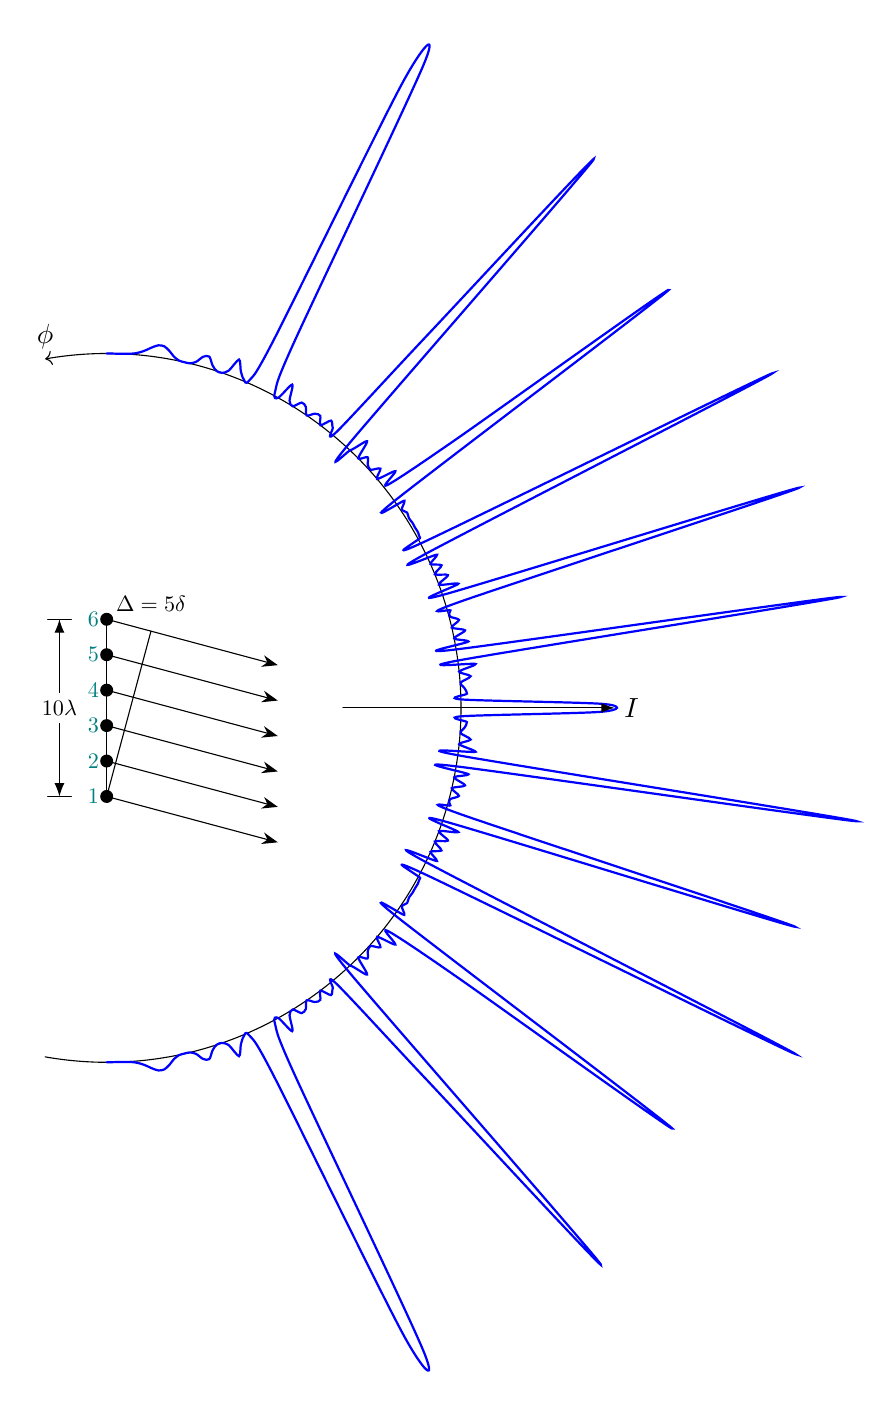
\begin{tikzpicture}[line cap=round, scale=1.5]
    % 관찰자가 움직일때의 도플러 효과
    \def\l{0.15}
    \def\th{15}
    \def\R{3}
    \def\ph{90}
    \def\k{8000}
    \coordinate (P1) at (0, {-\l*5});
    \coordinate (P2) at (0, {-\l*3});
    \coordinate (P3) at (0, {-\l*1});
    \coordinate (P4) at (0, {\l*1});
    \coordinate (P5) at (0, {\l*3});
    \coordinate (P6) at (0, {\l*5});
    \coordinate (A0) at ({-\ph-10}:\R); 

    \filldraw[] (P1) circle (0.05) node[left, scale=0.8, teal] {$1$};
    \filldraw[] (P2) circle (0.05) node[left, scale=0.8, teal] {$2$};
    \filldraw[] (P3) circle (0.05) node[left, scale=0.8, teal] {$3$};
    \filldraw[] (P4) circle (0.05) node[left, scale=0.8, teal] {$4$};
    \filldraw[] (P5) circle (0.05) node[left, scale=0.8, teal] {$5$};
    \filldraw[] (P6) circle (0.05) node[left, scale=0.8, teal] {$6$};

    \draw [] ($(P1) + (-0.3, 0)$) --($(P1) + (-0.5, 0)$);
    \draw [] ($(P6) + (-0.3, 0)$) --($(P6) + (-0.5, 0)$);
    \draw[Latex-Latex]($(P1) + (-0.4, 0)$) --node[ midway,fill=white, scale=0.8] {$10\lambda$} ($(P6) + (-0.4, 0)$);
    \draw[] (P1) -- (P6); 

    %\node[xshift=10, yshift=3] at (P1) {$\Delta$};
    \draw [] (P1) -- ++  ({90-\th}:{10*\l*cos(\th)}) node [yshift=10, scale=0.8] {$\Delta = 5\delta$};
    %\draw [] (P2) -- ++ ({90-\th}:{\l*12});
    
    \draw [-{Stealth[length=2mm]}] (P1) -- ++ (-\th: {\l*10});
    \draw [-{Stealth[length=2mm]}] (P2) -- ++ (-\th: {\l*10});
    \draw [-{Stealth[length=2mm]}] (P3) -- ++ (-\th: {\l*10});
    \draw [-{Stealth[length=2mm]}] (P4) -- ++ (-\th: {\l*10});
    \draw [-{Stealth[length=2mm]}] (P5) -- ++ (-\th: {\l*10});
    \draw [-{Stealth[length=2mm]}] (P6) -- ++ (-\th: {\l*10});



    \draw [->](A0) arc ({-\ph-10}:{\ph+10}:\R) node [above ]{$\phi$}; 
    \draw[domain={-\ph}:\ph,variable=\t,samples=200,smooth, thick,blue] 
        %\def\Q{{sin(2*\t) + \R}};
        plot (\t:{ \R+0.1*
        (
            (
                (1-cos(\k*(12*\l*sin(\t))))*(1-cos(\k*(2*\l*sin(\t))))+
                (sin(\k*(12*\l*sin(\t)))*sin(\k*(2*\l*sin(\t))))
                )/
            ((1-cos(\k*(2*\l*sin(\t))))^2+(sin(\k*(2*\l*sin(\t))))^2)
            )^2});
    
    \draw[-Latex] ({\R-1}, 0) -- ({\R+1.3}, 0) node [right] {$I$};
    \end{tikzpicture}
\end{document}
